\section{Introduction}

The general overview of the technical implementation is shown in Figure \ref{fig:docker_background2.pdf}. In the following subsections, we describe the deployment and testing architecture of generated code using system containers.





It is an operating system-level virtualization method for running multiple isolated Linux systems (containers) on a control host using a single Linux kernel. 
The Linux kernel provides the cgroups functionality that allows limitation and prioritization of resources (CPU, memory, block I/O, network, etc.) for each container without the need of starting any virtual machines~\cite{luotowards}.
These containers share the same OS and hardware as the hosting machine and it is very useful to use them in order to create new configurable and isolated instances to run. 
With container-based virtualization, we reduce the overhead associated with having each guest running a new installed operating system like using virtual machines. This approach can also improve the performance because there is just one operating system taking care of hardware calls.

%Thus, instead of configuring all code generators under test (GUTs) within the same host machine, we wrap each GUT within a system container. Afterwards, a new instance of the container is created to enable the execution of generated code in an isolated and configured environment. Meanwhile, we start our runtime testing components. A monitoring component collects usage statistics of all running containers and save them at runtime in a time series database component. Thus, we can compare later information about the resource usage of generated programs and detect inconsistencies within code generators.


\begin{figure*}[!h]
	\center
	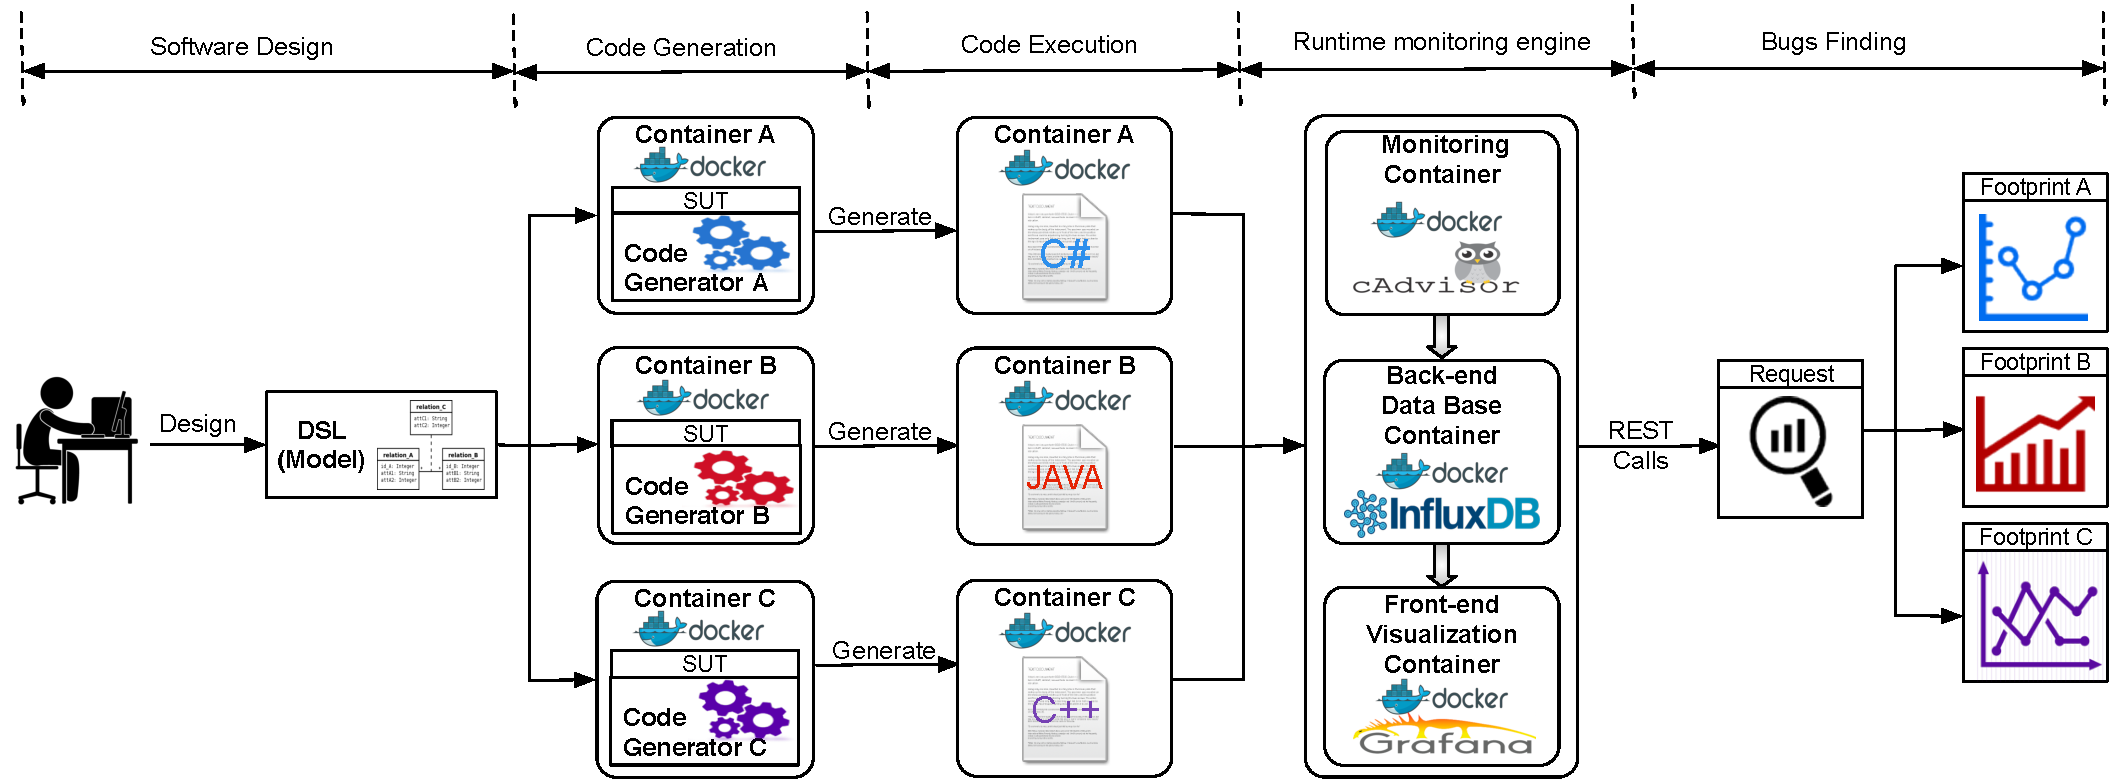
\includegraphics[width=0.95\linewidth]{chapitre5/fig/docker_background2.pdf}
	\caption{A technical overview of the different processes involved to ensure the code generation and non-functional testing of produced code from design time to runtime.}
	\label{fig:docker_background2.pdf}
\end{figure*}


\section{System Containers as Execution Platforms}


%For this purpose, we propose a testing infrastructure based on System Container techniques such as Docker\footnote{\url{https://www.docker.com}} environment. 
%This framework automates the deployment and execution of applications inside software containers by allowing multiple program configurations to run autonomously on different servers (i. e., a cloud servers).
%It also provides a distributed environment where system storage and resources can be finely managed and limited according to the needs. 

%Thus, we integrate a collection of components to define the adequate infrastructure for testing and monitoring of code generators. 


Before starting to monitor and test applications, we have to deploy generated code on different components to ease containers provisioning and profiling. 
We aim to use Docker Linux containers to monitor the execution of different generated artifacts in terms of resource usage~\cite{merkel2014docker}. 
Docker\footnote{\url{https://www.docker.com}} is an engine that automates the deployment of any application as a lightweight, portable, and self-sufficient container that runs virtually on a host machine. 
%To achieve that, Docker uses the Linux container technology. 
Using Docker, we can define pre-configured applications and servers to host as virtual images. We can also define the way the service should be deployed in the host machine using configuration files called Docker files. 
In fact, instead of configuring all code generators under test (GUTs) within the same host machine (as shown in Figure~1), our tool wrap each GUT within a container. To do so, we create a new configuration image for each GUT (i.e., the Docker image) where we install all the libraries, compilers, and dependencies needed to ensure the code generation and compilation. Thereby, the GUT produce code within multiple instances of preconfigured Docker images (see code generation step in Figure~2).
%As properties, we can define the OS where the service has to run, dependencies, etc. 
%A simple way to build images automatically is to use Dockerfiles which represents configuration files.
%Docker can build images automatically by reading the instructions from a Dockerfile. 
We use the public Docker registry\footnote{\url{https://hub.docker.com/}} for  saving, and managing all our Docker images. 
%It represents a cloud-based registry service for building and shipping application or service containers.
We can then instantiate different containers from these Docker images. 
%Basically, each container deploys an optimized version of the input source code program.

Next, each generated code is executed individually inside an isolated Linux container (see code execution step in Figure~2). By doing so, we ensure that each executed program runs in isolation without being affected by the host machine or any other processes. Moreover, since a container is cheap to create, we are able to create too many containers as long as we have new programs to execute.  
Since each program execution requires a new container to be created, it is crucial to remove and kill containers that have finished their job to eliminate the load on the system. We run the experiment on top of a private data-center that provide a bare-metal installation of  docker and docker swarm. On a single machine,  containers/softwares are running sequentially and we pin $p$ cores and $n$ Gbytes of memory for each container\footnote{$p$ and $n$ can be cofigured}. Once the execution is done, resources reserved for the container are automatically released to enable spawning next containers. Therefore, the host machine will not suffer too much from performance trade-offs.

In short, the main advantages of this approach are:
\begin{itemize}
	\item The use of containers induces less performance overhead and resource isolation compared to using a full stack virtualization solution~\cite{spoiala2016performance}. Indeed, instrumentation and monitoring tools for memory profiling like Valgrind~\cite{nethercote2007valgrind} can induce too much overhead.
	\item Thanks to the use of Dockerfiles, the proposed framework can be  configured by software testers in order to define the code generators under test (\eg, code generator version, dependencies, etc.), the host IP and OS, the DSL design, the optimization options, etc. Thus, we can use the same configured Docker image to execute different instances of generated code. For hardware architecture, containers share the same platform architecture as the host machine (e.g., x86, x64, ARM, etc.). 
	\item Docker uses Linux control groups (Cgroups) to group processes running in the container. This allows us to manage the resources of a group of processes, which is very valuable. 
	This approach increases the flexibility when we want to manage resources, since we can manage every group individually. For example, if we would evaluate the non-functional requirements of generated code within a resource-constraint environment, we can  request and limit resources within the execution container according to the needs.
	\item Although containers run in isolation, they can share data with the host machine and other running containers. Thus, non-functional data relative to resource consumption can be gathered and managed by other containers (\ie, for storage purpose, visualization)
\end{itemize}




\section{Runtime Testing Components}
In order to test our running applications within Docker containers, we aim to use a set of Docker components to ease the extraction of resource usage information (see runtime monitoring engine in Figure~2).
\subsection{Monitoring Component}
This container provides an understanding of the resource usage and performance characteristics of our running containers. Generally, Docker containers rely on Cgroups file systems to expose a lot of metrics about accumulated CPU cycles, memory, block I/O usage, etc. Therefore, our monitoring component automates the extraction of runtime performance metrics stored in Cgroups files. For example, we access live resource consumption of each container available at the Cgroups file system via stats found in \textit{"/sys/fs/cgroup/cpu/docker/(longid)/"} (for CPU consumption) and \textit{"/sys/fs/cgroup/memory/docker/(longid)/"} (for stats related to memory consumption). This component will automate the process of service discovery and metrics aggregation for each new container. Thus, instead of gathering manually metrics located in Cgroups file systems, it extracts automatically the runtime resource usage statistics relative to the running component (i.e., the generated code that is running within a container). We note that resource usage information is collected in raw data. This process may induce a little overhead because it does  very fine-grained accounting of resource usage on running container. Fortunately, this may not affect the gathered performance values since we run only one version of generated code within each container.
To ease the monitoring process, we integrate cAdvisor, a Container Advisor\footnote{\url{https://github.com/google/cadvisor}}. cAdvisor monitors service containers at runtime. 

However, cAdvisor monitors and aggregates live data over only 60 seconds interval. Therefore, we record all data over time, since container's creation, in a time-series database. It allows the code-generator testers to run queries and define non-functional metrics from historical data. Thereby, to make gathered data truly valuable for resource usage monitoring, we link our monitoring component to a back-end database component. 



\subsection{Back-end Database Component}
This component represents a time-series database back-end. It is plugged with the previously described monitoring component to save the non-functional data for long-term retention, analytics and visualization. 

During the execution of generated code, resource usage stats are continuously sent to this component. When a container is killed, we are able to access to its relative resource usage metrics through the database. We choose a time series database because we are collecting time series data that correspond to the resource utilization profiles of programs execution.

We use InfluxDB\footnote{\url{https://github.com/influxdata/influxdb}}, an open source distributed time-series database as a back-end to record data. InfluxDB allows the user to execute SQL-like queries on the database. For example, the following query reports the maximum memory usage of container $"generated\_code\_v1"$ since its creation:

\begin{lstlisting}[
language=SQL,
showspaces=false,
basicstyle=\small,
numberstyle=\small,
commentstyle=\color{gray},
linewidth=\columnwidth
]
select max (memory_usage) from stats 
where container_name='generated_code_v1'
\end{lstlisting}
To give an idea about the data gathered by the monitoring component and stored in the time-series database, we describe in Table \ref{tab:metrics} these collected metrics:
\begin{table}[h]
	\begin{center}
			\resizebox{0.8\columnwidth}{!}{%
		\begin{tabular}{|p{1.4cm}|p{6.6cm}|}
			\hline
			\textbf{Metric} & \textbf{Description} \\
				\hline
			Name & Container Name \\\hline
			
			T & Elapsed time since container's creation \\\hline
			
			Network  &  Stats for network bytes and packets in an out of the container \\\hline
			
			Disk IO &  Disk I/O stats \\\hline
			
			Memory  &  Memory usage \\\hline
			
			CPU &  CPU usage \\
			\hline
			
		\end{tabular}%
	}
		
	\end{center}
	\caption {Resource usage metrics recorded in InfluxDB}
	\label{tab:metrics}
\end{table}

Apart from that, our framework provides also information about the size of generated binaries and the compilation time needed to produce code.
For instance, resource usage statistics are collected and stored using these two components. It is relevant to show resource usage profiles of running programs overtime. To do so, we present a front-end visualization component for performance profiling. 

\subsection{Front-end Visualization Component}
%Once we gather and store resource usage data, the next step is visualizing them. That is the role of the visualization component. It will be the endpoint component that we use to visualize the recorded data. 
Once we gather and store resource usage data, the next step is visualizing them. That is the role of the visualization component. It will be the endpoint component that we use to visualize the recorded data. Therefore, we provide a dashboard to run queries and view different profiles of resource consumption of running components through web UI. Thereby, we can compare visually the profiles of resource consumption among containers. Moreover, we use this component to export the data currently being viewed into static CSV document. So, we can perform statistical analysis on this data to detect inconsistencies or performance anomalies (see bugs finding step in Figure~2).
%Moreover, we use this component to export the data currently being viewed into static CSV document. 
%Thereby, we can perform statistical analysis and process data to analyze performance behavior. 
%An overview of the monitoring dashboard is shown in Figure 3.
As a visualization component, we use Grafana\footnote{\url{https://github.com/grafana/grafana}}, a time-series visualization tool available for Docker. 


\begin{remark}
	We would notice that this testing infrastructure can be generalized and adapted to other case studies other than code generators. Using system containers, any software application/generated code can be easily deployed within containers (i.e., by configuring the container image). It will be later executed and monitored using our runtime monitoring engine. 
\end{remark}

 	

